\documentclass[12pt, a4paper]{article}

%----- 数学相关宏包 -----
\usepackage{amsmath}          % AMS 数学公式环境
\usepackage{amssymb}          % AMS 数学符号
\usepackage{amsfonts}         % AMS 数学字体
\usepackage{bm}               % 处理数学公式中的黑斜体
% Define bold vectors if desired for consistency
\newcommand{\vek}[1]{\mathbf{#1}}
%----- 页面与格式 -----
\usepackage[top=2.5cm, bottom=2.5cm, left=2.5cm, right=2.5cm]{geometry} % 页边距设置
\usepackage{graphicx}         % 插图
\usepackage{setspace}         % 设置行距,例如 \onehalfspacing
\usepackage{indentfirst}      % 首行缩进
\usepackage{titlesec}         % 自定义章节标题格式 (可选)

%----- 中文支持 -----
\usepackage{ctex}             % 中文支持宏包

%----- 其他常用宏包 -----
\usepackage{xcolor}           % 颜色支持 (可选)
\usepackage{hyperref}         % 超链接 (可选)
\hypersetup{
    colorlinks=true,
    linkcolor=blue,
    filecolor=magenta,
    urlcolor=cyan,
    citecolor=green,
}
%----- 绘图包 -----
\usepackage{tikz}
\usepackage{pgfplots}
\pgfplotsset{compat=1.18} % 建议使用较新的兼容版本

%----- 文档信息 -----
\title{固体物理作业}
\author{郑晓旸 202111030007} % 作者姓名和学号
\date{\today} % 或者指定日期 \date{2025年5月5日}

%----- 正文开始 -----
\begin{document}

\maketitle % 显示标题、作者、日期

\section*{问题与解答} % 使用无编号章节
\subsection*{问题 4.1}
根据 \(k = \pm \frac{\pi}{a}\) 状态简并微扰结果,求出与 \(E_-\) 及 \(E_+\) 相应的波函数 \(\psi_-\) 及 \(\psi_+\)。说明它们都代表驻波,并比较两个电子云分布(即 \(|\psi|^2\))说明能隙的来源(假设 \(V_n = V_n^*\))。

\subsection*{解答}
令 \(k = \frac{\pi}{a}\),\(k' = -\frac{\pi}{a}\),简并微扰波函数为 \(\psi = A\psi_k^0(x) + B\psi_{k'}^0(x)\)。
\[
\begin{cases}
[E^0(k) - E]A + V_n B = 0 \\
V_n^* A + [E^0(k') - E]B = 0
\end{cases}
\]
取 \(E = E_+\),带入上式,其中 \(E_+ = E^0(k) + |V_n|\)。

\(V(x) < 0\),\(V_n < 0\),从上式得到 \(B = -A\),于是
\[
\psi_+ = A[\psi_k^0(x) - \psi_{k'}^0(x)] = \frac{A}{\sqrt{L}} \left[ e^{i\frac{\pi}{a}x} - e^{-i\frac{\pi}{a}x} \right] = \frac{2A}{\sqrt{L}} \sin \frac{\pi}{a} x
\]

取 \(E = E_-\),\(E_- = E^0(k) - |V_n|\),\(V_n^* A = -V_n B\),得到 \(A = B\)。
\[
\psi_- = A[\psi_k^0(x) + \psi_{k'}^0(x)] = \frac{A}{\sqrt{L}} \left[ e^{i\frac{\pi}{a}x} + e^{-i\frac{\pi}{a}x} \right] = \frac{2A}{\sqrt{L}} \cos \frac{\pi}{a} x
\]

由教材可知,\(\psi_+\) 及 \(\psi_-\) 均为驻波。在驻波状态下,电子的平均速度 \(v(k)\) 为零。产生驻波因为电子波矢 \(k = \frac{\pi}{a}\) 时,电子波的波长 \(\lambda = \frac{2\pi}{k} = 2a\),恰好满足布拉格反射条件,这时电子波发生全反射,并与反射波形成驻波。由于两驻波的电子分布不同,所以对应不同本征能量。

\subsection*{问题 4.2}
写出在一维近自由电子近似,第 \(n\) 个能带(\(n = 1, 2, 3\))中,简约波矢 \(k = \frac{\pi}{2a}\) 的 0 级波函数。

\subsection*{解答}
\[
\psi_k^*(x) = \frac{1}{\sqrt{L}} e^{jkx} = \frac{1}{\sqrt{L}} e^{j\frac{\pi}{2a}x} e^{i\frac{2\pi}{a}mx} = \frac{1}{\sqrt{L}} e^{i\frac{\pi}{2a}x} \cdot e^{i\frac{2\pi}{a}mx} =  \frac{1}{\sqrt{L}} e^{i\frac{2\pi}{a}(m+\frac{1}{4})x}
\]

第一能带: \(m \cdot \frac{\pi}{2a} = 0\), \(m = 0\), \(\psi_k^*(x) = \frac{1}{\sqrt{L}} e^{i\frac{\pi}{2a}x}\)

第二能带: \(b = b'\) 则 \(b' \rightarrow b\), \(m \cdot \frac{2\pi}{a} = -\frac{2\pi}{a}\), 即 \(m = -1\), \(\psi_k^*(x) = \frac{1}{\sqrt{L}} e^{i\frac{3\pi}{2a}x}\)

第三能带: \(c' \rightarrow c\), \(m \cdot \frac{2\pi}{a} = \frac{2\pi}{a}\), 即 \(m = 1\), \(\psi_k^*(x) = \frac{1}{\sqrt{L}} e^{i\frac{\pi}{2a}x} \cdot e^{i\frac{2\pi}{a}x} = \frac{1}{\sqrt{L}} e^{i\frac{5\pi}{2a}x}\)

\subsection*{问题 4.3}
电子在周期场中的势能:
\[
V(x) =
\begin{cases}
\frac{1}{2}m\omega^2 [b^2 - (x - na)^2], & \text{当 } na - b \leq x \leq na + b \\
0, & \text{当 } (n-1)a + b \leq x \leq na - b
\end{cases}
\]
其中 \(a = 4b\),\(\omega\) 是常数。

(1) 试图画出势能曲线,并求其平均值。
(2) 用近自由电子近似模型求出晶体的第一个及第二个带隙宽度。

\subsection*{解答}
(1) 题目设势能曲线如下所示:
\begin{center} % 使图形居中
    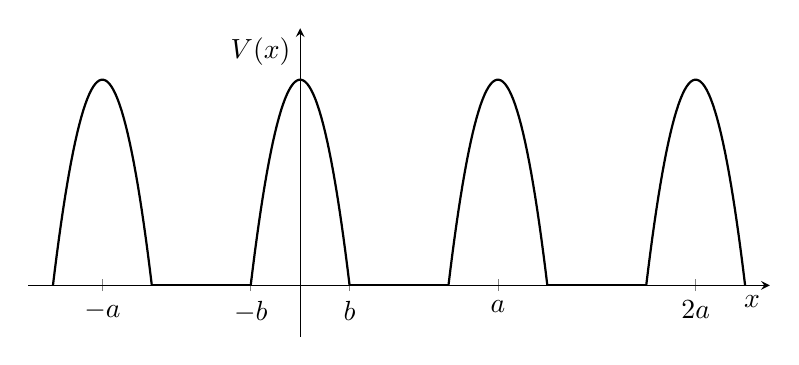
\begin{tikzpicture}
    \begin{axis}[
        axis lines=middle, % 坐标轴在原点交汇
        xlabel={$x$},      % x轴标签
        ylabel={$V(x)$},    % y轴标签
        xtick={-4, -1, 0, 1, 4, 8}, % x轴刻度位置 (基于 b=1, a=4)
        xticklabels={$-a$, $-b$, $0$, $b$, $a$, $2a$}, % x轴刻度标签
        ytick={0},          % y轴只在0处标记
        ymin=-0.5, ymax=2.5, % y轴范围 (Vmax设为2)
        xmin=-5.5, xmax=9.5, % x轴范围 (覆盖 -a-b 到 2a+b)
        width=11cm,        % 图形宽度
        height=5.5cm,       % 图形高度
        samples=50,         % 每个绘图段的采样点数,保证平滑
        xlabel style={anchor=north east}, % x轴标签位置
        ylabel style={anchor=north east}, % y轴标签位置
        clip=false          % 允许绘制超出坐标轴范围
    ]
    
    % --- 定义参数 (为了绘图方便,设 b=1, a=4b=4, 峰值 Vmax=2) ---
    \def\myb{1}
    \def\mya{4}
    \def\myVmax{2} % 对应 C*b^2 = (1/2)m*omega^2*b^2
    
    % --- 绘制各段势能曲线 ---
    % n = -1 抛物线段 (区间 [-a-b, -a+b] = [-5, -3])
    \addplot[black, thick, domain=-\mya-\myb:-\mya+\myb] {\myVmax * (1 - (x + \mya)^2 / (\myb^2))};
    % 零势能段 (区间 [-a+b, -b] = [-3, -1])
    \addplot[black, thick, domain=-\mya+\myb:-\myb] {0};
    % n = 0 抛物线段 (区间 [-b, b] = [-1, 1])
    \addplot[black, thick, domain=-\myb:\myb] {\myVmax * (1 - x^2 / (\myb^2))};
    % 零势能段 (区间 [b, a-b] = [1, 3])
    \addplot[black, thick, domain=\myb:\mya-\myb] {0};
    % n = 1 抛物线段 (区间 [a-b, a+b] = [3, 5])
    \addplot[black, thick, domain=\mya-\myb:\mya+\myb] {\myVmax * (1 - (x - \mya)^2 / (\myb^2))};
    % 零势能段 (区间 [a+b, 2a-b] = [5, 7])
    \addplot[black, thick, domain=\mya+\myb:2*\mya-\myb] {0};
    % n = 2 抛物线段 (区间 [2a-b, 2a+b] = [7, 9])
    \addplot[black, thick, domain=2*\mya-\myb:2*\mya+\myb] {\myVmax * (1 - (x - 2*\mya)^2 / (\myb^2))};
    
    % --- 添加中心虚线 (从原点到 Vmax) ---
    \draw [dashed] (axis cs:0, 0) -- (axis cs:0, \myVmax);
    
    \end{axis}
    \end{tikzpicture}
\end{center}    


(2) 势的平均值:由图可见,\(V(x)\) 是一个以 \(a\) 为周期的周期函数,所以
\[
\overline{V(x)} = \frac{1}{L} \int V(x) dx = \frac{1}{a} \int_0^a V(x) dx = \frac{1}{a} \int V(x) dx
\]
题目设 \(a = 4b\),故积分上限应为 \(a - b = 3b\),但由于在 \([b, 3b]\) 区间内 \(V(x) = 0\),故只需在 \([-b, b]\) 区间内积分。这时,\(n = 0\),于是
\[
\overline{V} = \frac{1}{a} \int_{-b}^b V(x) dx = \frac{m\omega^2}{2a} \int_{-b}^b (b^2 - x^2) dx = \frac{m\omega^2}{2a} \left[ b^2 x - \frac{1}{3} x^3 \right]_{-b}^b = \frac{1}{6} m\omega^2 b^2
\]

(3) 势能在 \([-2b, 2b]\) 区间是个偶函数,可以展开成傅里叶级数
\[
V(x) = V_0 + \sum_{m = -\infty}^{\infty} V_m \cos \frac{m\pi}{2b} x, \quad V_m = \frac{2}{2b} \int_0^{2b} V(x) \cos \frac{m\pi}{2b} x dx = \frac{1}{b} \int_0^b V(x) \cos \frac{m\pi}{2b} x dx
\]

第一个禁带宽度 \(E_{g1} = 2|V_1|\),以 \(m = 1\) 代入上式,
\[
E_{g1} = \frac{m\omega^2}{b} \int_0^b (b^2 - x^2) \cos \frac{\pi x}{2b} dx
\]
利用积分公式 \(\int u^2 \cos mu du = \frac{u}{m^2} (mu \sin mu + 2 \cos mu) - \frac{2}{m^3} \sin mu\) 得
\[
E_{g1} = \frac{16 m\omega^2}{\pi^3} b^2
\]
第二个禁带宽度 \(E_{g2} = 2|V_2|\),以 \(m = 2\) 代入上式,代入上式
\[
E_{g2} = \frac{m\omega^2}{b} \int_0^b (b^2 - x^2) \cos \frac{\pi x}{b} dx
\]
再次利用积分公式有
\[
E_{g2} = \frac{2 m\omega^2}{\pi^2} b^2
\]

\subsection*{问题 4.12}
设有二维正方晶格,晶体势为 \(U(x,y) = -4U \cos\left(\frac{2\pi x}{a}\right) \cos\left(\frac{2\pi y}{a}\right)\)。
用近自由电子近似的微扰论,近似求出布里渊区顶角 \((\frac{\pi}{a}, \frac{\pi}{a})\) 处的能隙。
\subsection*{解答}
以 \(\hat{\mathbf{i}}, \hat{\mathbf{j}}\) 表示位置矢量的单位矢量,以 \(\hat{\mathbf{b}}_1, \hat{\mathbf{b}}_2\) 表示倒易矢量的单位矢量,则有,
\( \vek{r} = x\hat{\mathbf{i}} + y\hat{\mathbf{j}} \), \( \vek{G} = G_1\hat{\mathbf{b}}_1 + G_2\hat{\mathbf{b}}_2 = \frac{2\pi}{a}(g_1\hat{\mathbf{b}}_1 + g_2\hat{\mathbf{b}}_2) \), \( g_1, g_2 \) 为整数。
晶体势能 \( U(x,y) = -4U \cos\left(\frac{2\pi x}{a}\right) \cos\left(\frac{2\pi y}{a}\right) \)。
可以写成傅里叶级数形式:
\[
U(\vek{r}) = -U \left( e^{i\frac{2\pi}{a}x} + e^{-i\frac{2\pi}{a}x} \right) \left( e^{i\frac{2\pi}{a}y} + e^{-i\frac{2\pi}{a}y} \right) = \sum_{\vek{G}} U_{\vek{G}} e^{i\vek{G}\cdot \vek{r}}
\]
其中非零的傅里叶系数为 \( U_{\vek{G}(1,1)} = U_{\vek{G}(-1,-1)} = U_{\vek{G}(1,-1)} = U_{\vek{G}(-1,1)} = -U \)。 (注:这里 \(\vek{G}(g_1, g_2)\) 表示 \(g_1\frac{2\pi}{a}\hat{\mathbf{b}}_1 + g_2\frac{2\pi}{a}\hat{\mathbf{b}}_2\) 对应的倒格矢,其系数为 \(U_{\vek{G}}\)。)
基本方程为
\[
(\lambda_{\vek{K}} - \epsilon)C(\vek{K}) + \sum_{\vek{G}} U_{\vek{G}} C(\vek{K}-\vek{G}) = 0
\]
其中 \( \lambda_{\vek{K}} = \frac{\hbar^2 K^2}{2m} \)。
考虑布里渊区顶角 \( \vek{K} = (\frac{\pi}{a}, \frac{\pi}{a}) \)。 这个波矢与 \( \vek{K}' = \vek{K} - \vek{G}(1,1) = (\frac{\pi}{a}, \frac{\pi}{a}) - (\frac{2\pi}{a}, \frac{2\pi}{a}) = (-\frac{\pi}{a}, -\frac{\pi}{a}) = -\vek{K} \) 是简并的(在空晶格近似下,\( \lambda_{\vek{K}} = \lambda_{-\vek{K}} \))。
根据近自由电子近似的微扰论(特别是二能级近似),我们主要考虑这两个状态的耦合。其他 \( \vek{K} - \vek{G} \) 的能量 \( \lambda_{\vek{K}-\vek{G}} \) 与 \( \lambda_{\vek{K}} \) 相差较大。
与 \( C(\vek{K}) \) 耦合的主要项是 \( U_{\vek{G}(1,1)} C(\vek{K}-\vek{G}(1,1)) = U_{\vek{G}(1,1)} C(-\vek{K}) \)。
与 \( C(-\vek{K}) \) 耦合的主要项是 \( U_{\vek{G}(-1,-1)} C(-\vek{K}-\vek{G}(-1,-1)) = U_{\vek{G}(-1,-1)} C(\vek{K}) \)。
注意 \( U_{\vek{G}(1,1)} = U_{\vek{G}(-1,-1)} = -U \)。
因此,方程组简化为:
\[
\begin{cases}
(\lambda_{\vek{K}} - \epsilon)C(\vek{K}) + U_{\vek{G}(1,1)} C(-\vek{K}) = 0 \\
(\lambda_{-\vek{K}} - \epsilon)C(-\vek{K}) + U_{\vek{G}(-1,-1)} C(\vek{K}) = 0
\end{cases}
\]
即
\[
\begin{cases}
(\lambda_{\vek{K}} - \epsilon)C(\vek{K}) - U C(-\vek{K}) = 0 \\
(\lambda_{\vek{K}} - \epsilon)C(-\vek{K}) - U C(\vek{K}) = 0
\end{cases}
\]
该线性方程组有非零解的条件是系数行列式为零:
\[
\begin{vmatrix}
\lambda_{\vek{K}} - \epsilon & -U \\
-U & \lambda_{\vek{K}} - \epsilon
\end{vmatrix} = 0
\]
其中
\[
\lambda_{\vek{K}} = \frac{\hbar^2 |\vek{K}|^2}{2m} = \frac{\hbar^2}{2m} \left[ \left(\frac{\pi}{a}\right)^2 + \left(\frac{\pi}{a}\right)^2 \right] = \frac{\hbar^2 \pi^2}{ma^2}
\]
(注:图片中 \(\lambda\) 的计算步骤有歧义,这里给出详细过程)
行列式展开得到:
\[
(\lambda_{\vek{K}} - \epsilon)^2 - U^2 = 0
\]
解得能量本征值:
\[
\epsilon = \lambda_{\vek{K}} \pm U = \frac{\hbar^2 \pi^2}{ma^2} \pm U
\]
所以在布里渊区顶角 \( (-\frac{\pi}{a}, \frac{\pi}{a}) \) 处的两个能级为 \( \epsilon_+ = \frac{\hbar^2 \pi^2}{ma^2} + U \) 和 \( \epsilon_- = \frac{\hbar^2 \pi^2}{ma^2} - U \)。
能隙宽度为:
\[
\Delta\epsilon = \epsilon_+ - \epsilon_- = 2U
\]

\subsection*{问题 5.1}
设一维晶体的电子能带可以写成
\[
E(k) = \frac{\hbar^2}{ma^2} \left( -\frac{7}{8} \cos ka + \frac{1}{8} \cos 2ka \right)
\]
其中 \(a\) 为晶格常数,计算:
\begin{enumerate}
    \item 能带的宽度
    \item 电子在波矢 \(k\) 的状态时的速度
    \item 能带底部和能带顶部电子的有效质量
\end{enumerate}
\subsection*{解答}
\begin{enumerate}
    \item 能带的宽度的计算
    \[
    E(k) = \frac{\hbar^2}{ma^2} \left( -\frac{7}{8} \cos ka + \frac{1}{8} \cos 2ka \right)
    \]
    能带底部 \(k = 0\)
    \[
    E(0) = \frac{\hbar^2}{ma^2} \left( -\frac{7}{8} + \frac{1}{8} \right) = -\frac{3}{4} \frac{\hbar^2}{ma^2}
    \]
    能带顶部 \(k = \frac{\pi}{a}\)
    \[
    E\left(\frac{\pi}{a}\right) = \frac{\hbar^2}{ma^2} \left( -\frac{7}{8} \cos \pi + \frac{1}{8} \cos 2\pi \right) = \frac{\hbar^2}{ma^2} \left( \frac{7}{8} + \frac{1}{8} \right) = \frac{\hbar^2}{ma^2}
    \]
    能带宽度
    \[
    \Delta E = E\left(\frac{\pi}{a}\right) - E(0) = \frac{\hbar^2}{ma^2} - \left(-\frac{3}{4} \frac{\hbar^2}{ma^2}\right) = \frac{7}{4} \frac{\hbar^2}{ma^2}
    \]
    \item 电子在波矢 \(k\) 的状态时的速度
    \[
    E(k) = \frac{\hbar^2}{ma^2} \left( -\frac{7}{8} \cos ka + \frac{1}{8} \cos 2ka \right)
    \]
    电子的速度
    \[
    v(k) = \frac{1}{\hbar} \frac{dE(k)}{dk}
    \]
    \[
    v(k) = \frac{1}{\hbar} \frac{\hbar^2}{ma^2} \left( \frac{7}{8} a \sin ka - \frac{1}{8} 2a \sin 2ka \right) = \frac{\hbar}{ma} \left( \frac{7}{8} \sin ka - \frac{1}{4} \sin 2ka \right)
    \]
    \item 能带底部和能带顶部电子的有效质量
    \[
    E(k) = \frac{\hbar^2}{ma^2} \left( -\frac{7}{8} \cos ka + \frac{1}{8} \cos 2ka \right)
    \]
    电子的有效质量
    \[
    m^* = \hbar^2 \left/ \frac{\partial^2 E}{\partial k^2} \right.
    \]
    \[
    \frac{\partial^2 E}{\partial k^2} = \frac{\hbar^2}{ma^2} \left( -\frac{7}{8} (-a^2) \cos ka + \frac{1}{8} (-4a^2) \cos 2ka \right) = \frac{\hbar^2}{m} \left( \frac{7}{8} \cos ka - \frac{1}{2} \cos 2ka \right)
    \]
    \[
    m^* = \frac{\hbar^2}{\frac{\hbar^2}{m} \left( \frac{7}{8} \cos ka - \frac{1}{2} \cos 2ka \right)} = \frac{m}{\frac{7}{8} \cos ka - \frac{1}{2} \cos 2ka}
    \]
    能带底部 \(k = 0\)
    \[
    m^* = \frac{m}{\frac{7}{8} - \frac{1}{2}} = \frac{m}{\frac{3}{8}} = \frac{8}{3} m
    \]
    能带顶部 \(k = \frac{\pi}{a}\)
    \[
    m^* = \frac{m}{\frac{7}{8} \cos \pi - \frac{1}{2} \cos 2\pi} = \frac{m}{-\frac{7}{8} - \frac{1}{2}} = \frac{m}{-\frac{11}{8}} = -\frac{8}{11} m
    \]
\end{enumerate}
% 请将具体的问题和解答内容放在这里

\end{document}
%----- 正文结束 -----
